\documentclass[11pt]{article}
\usepackage[T1]{fontenc}
\usepackage{lmodern}
\usepackage[margin=1in]{geometry}
\usepackage{amsmath,amssymb}
\usepackage{microtype}
\usepackage{graphicx}
\usepackage{tabularx}
\usepackage{xurl}
\usepackage[hidelinks]{hyperref}

\title{Assignment 2: Paper 1\\[0.4em]
\large Understanding Deep Learning Requires Rethinking Generalization}
\author{Jireh Katebe}
\date{CS 6362 Advanced Machine Learning, Fall 2026\\22 October 2026}

\begin{document}
\maketitle

\section{Problem statement and understanding of the methodology}

\subsection{The problem and intuition}

The authors ask why deep neural networks can generalise despite having enough capacity to memorise their training data~\cite{zhang2017}. These networks can have many more parameters than training examples and can fit arbitrary label assignments. When trained with correct labels, the same architectures can perform well on unseen examples. The paper investigates what accounts for this difference in test performance.

Regularisation is one proposed explanation for why networks with more parameters than training examples generalise. The authors examine this explanation by removing explicit regularisers and measuring performance. The models still generalise, although their accuracy can fall. The authors also randomise labels and inputs to test whether the training procedure can fit data whose class information has been disrupted.

\subsection{Mathematical formulation}

Following the lecture formulation, let $S=\{(x_i,y_i)\}_{i=1}^{n}$ contain $n$ training examples sampled independently from a distribution $\mathcal{D}$. Each input $x_i\in\mathbb{R}^{d}$ has $d$ features, and its label $y_i\in\{1,\ldots,K\}$ identifies one of $K$ classes. Let $f_w$ be the network, with parameters $w\in\mathbb{R}^{P}$, and let $\ell(f_w(x),y)$ measure its prediction loss. The expected and empirical risks are
\[
R(w)=\mathbb{E}_{(x,y)\sim\mathcal{D}}[\ell(f_w(x),y)],
\qquad
R_S(w)=\frac{1}{n}\sum_{i=1}^{n}\ell(f_w(x_i),y_i).
\]
Training aims to minimise $R_S(w)$. The goal is low expected risk $R(w)$, which measures performance on the underlying distribution. A held-out test set estimates this performance, and $R(w)-R_S(w)$ is the generalisation gap. The paper studies networks that can fit arbitrary training labels even when $P>n$. Their good test performance on correctly labelled data raises the question of what determines whether fitting the training set leads to generalisation.

\subsection{How the authors test it}

For the CIFAR-10 experiments in Figure 1, the authors use small Inception, small AlexNet, and a one-hidden-layer MLP. CIFAR-10 contains ten classes, with 50,000 training images and 10,000 test images.

For label corruption, draw $b_i\sim\operatorname{Bernoulli}(p)$ and an independent class $u_i\sim\operatorname{Uniform}\{1,\ldots,K\}$ for each example, where $p\in[0,1]$ is the corruption probability. The training target is
\[
\widetilde y_i=\begin{cases}y_i,&b_i=0,\\u_i,&b_i=1,\end{cases}
\qquad
\Pr(\widetilde y_i\ne y_i)=p\frac{K-1}{K}=0.9p.
\]
The last equality uses CIFAR-10's ten classes. Labels are drawn once and fixed across epochs. Redrawing them would give each image changing targets, so the experiment would no longer test memorisation of one fixed assignment. At $p=1$, the training labels are independent of the images. Chance performance on the balanced test set is $1/K=10\%$ accuracy, or $1-1/K=90\%$ error; individual runs can differ from this value.

Training uses cross-entropy with the assigned targets. Figure 1(c) uses classification error: training predictions are compared with $\widetilde y_i$, and test predictions with the original labels of unseen images. If $\widehat e_{\rm train}$ and $\widehat e_{\rm test}$ denote these two error rates, the plotted test-minus-training difference is $\widehat e_{\rm test}-\widehat e_{\rm train}=\widehat e_{\rm test}$ when training error is zero. Under corruption, this comparison uses different training and test label distributions.

The input-corruption experiments retain the original labels. For shuffled pixels, one permutation is applied to every image; for random pixels, each image has its own permutation. The Gaussian condition replaces images with noise matching the original data's mean and variance. These transformed training inputs stay fixed across epochs.

Figure 1(a) compares Inception's training loss under these three input changes, true labels, and random labels. Panel (b) compares the three architectures' fitting time as label corruption increases, relative to their clean-label baseline. Panel (c) shows their test error. The networks fit both correct and random labels, while test error increases with label corruption.

The broader argument combines these experiments with theory. Theorem 1 constructs a two-layer ReLU network with $2n+d$ weights that represents any real-valued targets on $n$ distinct inputs in $\mathbb{R}^d$. This establishes fitting capacity; the experiments test whether optimisation finds such fits. Table 1 shows generalisation without explicit regularisers, while their removal lowers ImageNet top-1 accuracy from 77.84\% to 59.80\%. Section 5 gives a possible role for optimisation: for a full-row-rank linear data matrix $X\in\mathbb{R}^{n\times d}$ and targets $y\in\mathbb{R}^n$, SGD initialised at zero stays in the span of the training inputs. If it reaches $Xw=y$, it selects the minimum-norm solution $w=X^\top(XX^\top)^{-1}y$. This illustrates implicit regularisation in linear models; the corresponding explanation for the tested nonlinear networks remains open.

\clearpage
\section{Reproduction of Figure 1}

I used ChatGPT, model Astra, to develop the PyTorch notebook. The shared page records the model identifier \texttt{gpt-6-astra-wm}.

\noindent Conversation: \url{https://chatgpt.com/share/6ada9094-f644-83e9-86ec-d563eff6b4b3}\\
Notebook: \path{figure1_reproduction.ipynb}\\
GitHub repository: \url{https://github.com/Jireh1226/AdvancedML_assignements}\\
Submission folder: \path{Assignment_2/paper_1_generalization/}.

\subsection{Phase 1: understanding the paper and asking for code}

I gave the LLM the paper, summarised my understanding, and asked it to check my interpretation. When its explanation differed from mine, I asked for the relevant section and went back to the paper to check the correction. Once the setup was clear, I requested the notebook in stages and checked the generated code against the paper. Settings absent from the paper were recorded as implementation assumptions.

\subsection{Phase 2: reviewing the LLM's output}

Remote-machine setup and transfer instructions were removed from the submitted notebook. In the code, a plotting cell could overwrite the clean baseline by assigning another experiment's history to the true-label curve. Plotting was separated from saving, and each run's results were stored independently. To resume interrupted runs consistently, checkpoints were extended to include the optimiser, scheduler, progress, history, and random-generator states alongside the weights.

After 64 epochs, 18 of 36 runs still had nonzero training error at the final checkpoint. Panel (b) also hid valid first-fit times whenever the final checkpoint had nonzero training error. The plot was corrected to use the recorded first-fit step, with final fitting checked separately.

Panel (a) used default colours rather than the paper's colours, including purple instead of black for Gaussian inputs; this presentation mismatch remains in the saved figure.

\subsection{Phase 3: running, correcting, and comparing the results}

\subsubsection{Settings used in the attempt}

The reproduction used all 50,000 CIFAR-10 training images and 10,000 test images. Panel (a) used the five Inception conditions. Panels (b,c) used Inception, AlexNet, and a one-hidden-layer MLP with 512 units, each at $p=0,0.1,\ldots,1$. Sharing the two Inception label endpoints between panels gave 36 unique configurations.

The saved parameter counts match Table 1: 1,649,402 for Inception, 1,387,786 for AlexNet, and 1,209,866 for MLP 1$\times$512. Matching counts check the architecture sizes, but do not establish identical padding or normalisation behaviour.

I instructed the LLM to use seed 42 because I considered it a common machine-learning default and hoped it might give results closer to the paper's. The paper does not report its seed; this choice provides repeatability, with no established advantage for matching its results. All runs used this one seed and batch size 128.

Images were centre-cropped to $28\times28$, scaled by $1/255$, transformed for the selected condition, and standardised separately using each image's mean and adjusted standard deviation.

Pixel permutations operated on all scalar channel values. Gaussian inputs used the cropped training data's global mean, approximately 0.46773, and variance, approximately 0.061063, before standardisation. The paper leaves permutation granularity and the calculation of these statistics open, so both are implementation assumptions.

The models used cross-entropy on raw logits. Following Appendix A, SGD used momentum 0.9, initial learning rates of 0.1 for Inception and 0.01 for AlexNet and the MLP, and a decay factor of 0.95 per epoch. There was no augmentation, dropout, or weight decay. Xavier-uniform initialisation, batch size, and the remaining padding and normalisation details were recorded implementation choices. The initial 64 epochs gave $64\lceil50000/128\rceil=25{,}024$ updates, close to panel (a)'s displayed range.

\begin{table}[htbp]
\centering\small
\begin{tabularx}{\textwidth}{@{}>{\raggedright\arraybackslash}X>{\raggedright\arraybackslash}X>{\raggedright\arraybackslash}X@{}}
\hline
Stated by the authors & Assumed in the implementation & Changed after failure \\
\hline
SGD momentum 0.9; initial rates 0.1/0.01; decay 0.95 per epoch & Batch 128; seed 42; Xavier-uniform initialisation; initial budget 64 epochs & AlexNet/MLP runs with residual errors continued at the epoch-64 rate \\
Centre crop to $28\times28$; scale and standardise each image; no explicit regularisers for randomisation tests & Scalar-channel permutations; global Gaussian moments; padding and BN/LRN conventions & No data, architecture, or corruption changes \\
Relative convergence time; zero training error stated in the Figure 1 caption & First epoch-end zero-error evaluation; 100-update loss averages & First-fit plotting gate corrected; relaxed thresholds used only for diagnostics \\
\hline
\end{tabularx}
\caption{Provenance of the main settings. Assumptions are distinct from later corrections.}
\end{table}

For panel (b), I defined $T(p)$ as the update count at the first epoch-end evaluation with exactly zero errors on all training examples. The plotted slowdown is $T(p)/T(0)$ for each architecture. Panel (c) uses test error from the final selected fitted checkpoint. Panel (a) uses sample-weighted loss averages over 100 updates.

\subsubsection{Failed attempts and corrections}

After 64 epochs, seven AlexNet runs and all eleven MLP runs still had training errors. The fully random-label MLP had 559 mistakes. Continuing it to 128 epochs with the original decay reduced this to 337, so doubling the budget still failed the zero-error criterion.

The 64-epoch budget came from panel (a)'s displayed range. The LLM had identified it as a starting choice, with no guarantee that every architecture would fit. By epoch 128, repeated multiplication by 0.95 had reduced the MLP learning rate to about $1.48\times10^{-5}$. This small rate motivated a constant-rate continuation. The failed extension showed that the original decay had not reached zero error within the tested budget; other causes of incomplete fitting remained possible.

The 18 unfinished runs were then continued from their original epoch-64 checkpoints, preserving the data, weights, momentum, and random states. After epoch 64, their learning rate was held at $0.01(0.95)^{64}\approx3.7524\times10^{-4}$. Each stopped at the first subsequent zero-error evaluation, with a 1,024-epoch safety cap. This learning-rate floor changes the paper's schedule. The resulting AlexNet/MLP curves are a modified-protocol reproduction. Inception and panel (a) retain the original schedule.

All 18 continued runs fitted before the safety cap. Some AlexNet runs had already reached zero errors before making one error at epoch 64. Their earlier fitting times had been hidden by the plotting rule described in Phase 2. Panel (b) now keeps the first zero-error timestamp, while panel (c) uses the final fitted checkpoints.

Smaller batches were also tested with the original exponential decay. With batch 32, the MLP still had 91 random-label training errors after 128 epochs. Batch 16 left four errors even on clean labels. AlexNet with batch 32 fitted every level $p\leq0.8$ within 64 epochs and gave an endpoint slowdown of $62/22=2.818$, but $p=0.9$ retained two errors after 128 epochs. Since every corruption level had to reach zero errors, the entire replacement sweep was rejected. The runs with the constant-rate continuation were retained.

\subsubsection{Results, differences, and what they support}

\begin{table}[htbp]
\centering
\small
\begin{tabular}{lrrrr}
\hline
Model & Clean test & Random test & First-fit epochs & $T(1)/T(0)$ \\
 & accuracy (\%) & accuracy (\%) & clean/random & \\
\hline
Inception & 86.52 & 9.97 & 14/46 & 3.286 \\
AlexNet & 76.52 & 9.93 & 15/83 & 5.533 \\
MLP 1$\times$512 & 50.72 & 9.90 & 393/458 & 1.165 \\
\hline
\end{tabular}
\caption{Selected clean-label and fully resampled-label results. All selected configurations have zero final training errors. First-fit epochs can precede the end of a run.}
\label{tab:paper1-results}
\end{table}

All five Inception conditions reach low training loss in panel (a), with random labels taking longest to fit. In panel (c), test error approaches 90\% as label corruption increases. The larger mismatch is in the reproduced panel (b): AlexNet's slowdown exceeds Inception's, and the MLP ratios are low and non-monotonic. The paper places AlexNet below the other two models. Figures~\ref{fig:paper1-original} and~\ref{fig:paper1-reproduction} show the original and reproduced curves.

\begin{figure}[!t]
\centering
\includegraphics[page=4,trim=107bp 580bp 107bp 78bp,clip,width=\textwidth]{259_understanding_deep_learning_re.pdf}
\caption{Original Figure 1, cropped from the supplied paper~\cite{zhang2017}.}
\label{fig:paper1-original}
\end{figure}

\begin{figure}[p]
\centering
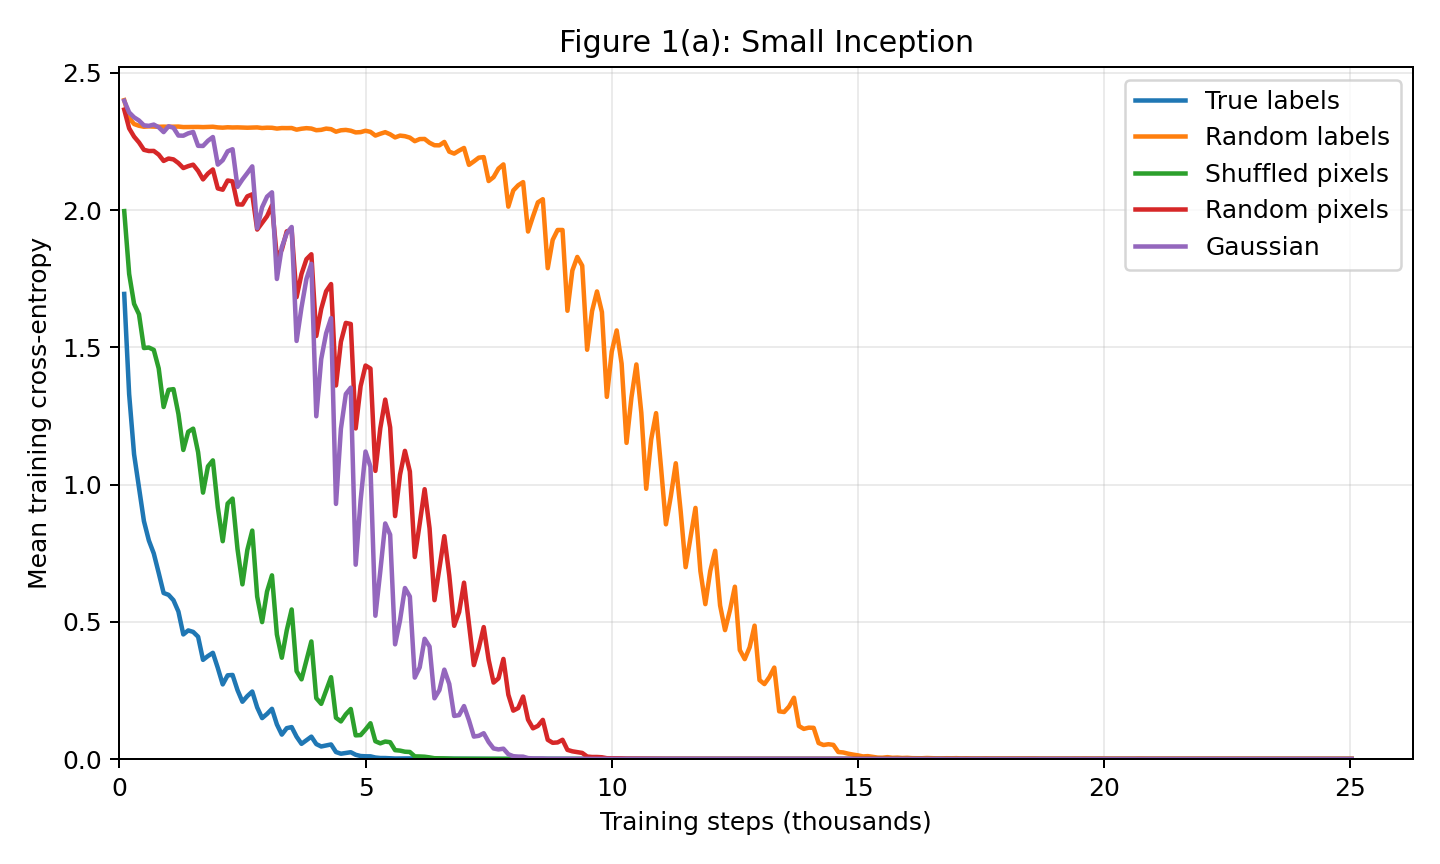
\includegraphics[width=0.76\textwidth]{results_figure1_reviewed/full/figure1a.png}
\par\medskip
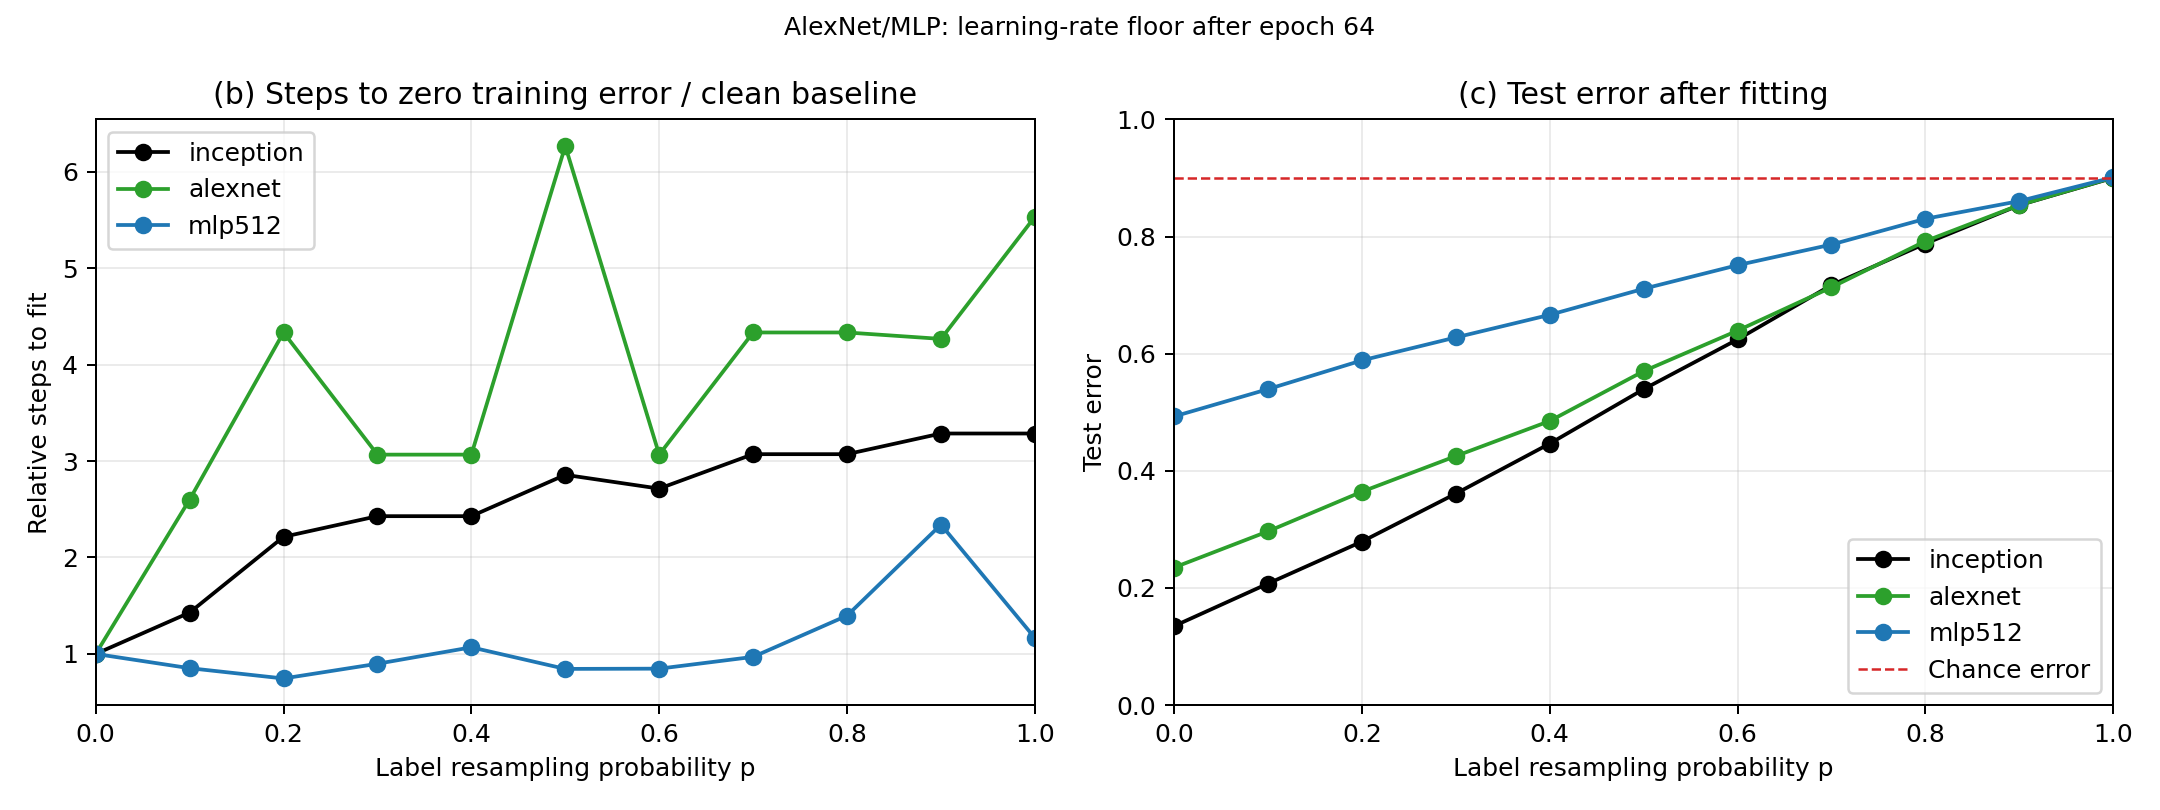
\includegraphics[width=\textwidth]{results_figure1_reviewed/full/figure1bc.png}
\caption{Reproduced Figure 1: panel (a) above and panels (b,c) below. The saved plots are enlarged without changing their measurements or smoothing. AlexNet/MLP continuations use the disclosed learning-rate floor; Inception retains the original schedule.}
\label{fig:paper1-reproduction}
\end{figure}

The saved histories identify a substantial source of timing sensitivity: the last training error can persist long after most examples are fitted. The clean MLP has one error at every evaluation from epochs 175 through 392, then reaches zero at epoch 393. AlexNet at $p=0.5$ has one error from epochs 42 through 93, reaching zero at 94. AlexNet at $p=0.4$ reaches zero at epoch 46, then returns to one error at epochs 47--65. The last case also shows why the first-fit timestamp and final fitting status must be checked separately. These counts do not establish that the same example was misclassified at every epoch.

To measure this sensitivity, I recomputed the first fitting time from each saved history at three thresholds. Let $T_\epsilon(p)$ be the first epoch-end step with training error at most $\epsilon$. Table~\ref{tab:threshold-sensitivity} reports endpoint times and $T_\epsilon(1)/T_\epsilon(0)$. Only the evaluation threshold changes; the selected trajectories are identical.

\begin{table}[htbp]
\centering\small
\begin{tabular}{lrrr}
\hline
Model & At least 99\% & At least 99.9\% & Exactly 100\% \\
\hline
Inception & 12/38 (3.167) & 13/38 (2.923) & 14/46 (3.286) \\
AlexNet & 12/31 (2.583) & 14/34 (2.429) & 15/83 (5.533) \\
MLP 1$\times$512 & 25/68 (2.720) & 37/201 (5.432) & 393/458 (1.165) \\
\hline
\end{tabular}
\caption{Clean/random first-fit epochs, followed by the slowdown ratio in parentheses. Thresholds allow 500, 50, or zero errors among 50,000 examples. These are diagnostics, not replacement training runs.}
\label{tab:threshold-sensitivity}
\end{table}

At the 99\% threshold, the endpoint ordering becomes Inception, MLP, then AlexNet, as in the paper. This does not hold uniformly across the grid: the MLP and AlexNet curves cross, and the MLP ratio falls slightly from 2.76 at $p=0.9$ to 2.72 at $p=1$. AlexNet's endpoint is also above the paper's approximately 1.5. The supplementary curve in Figure~\ref{fig:threshold-sensitivity} therefore shows improved agreement in some features, with remaining differences. The primary reproduction keeps the exact-zero definition.

\begin{figure}[htbp]
\centering
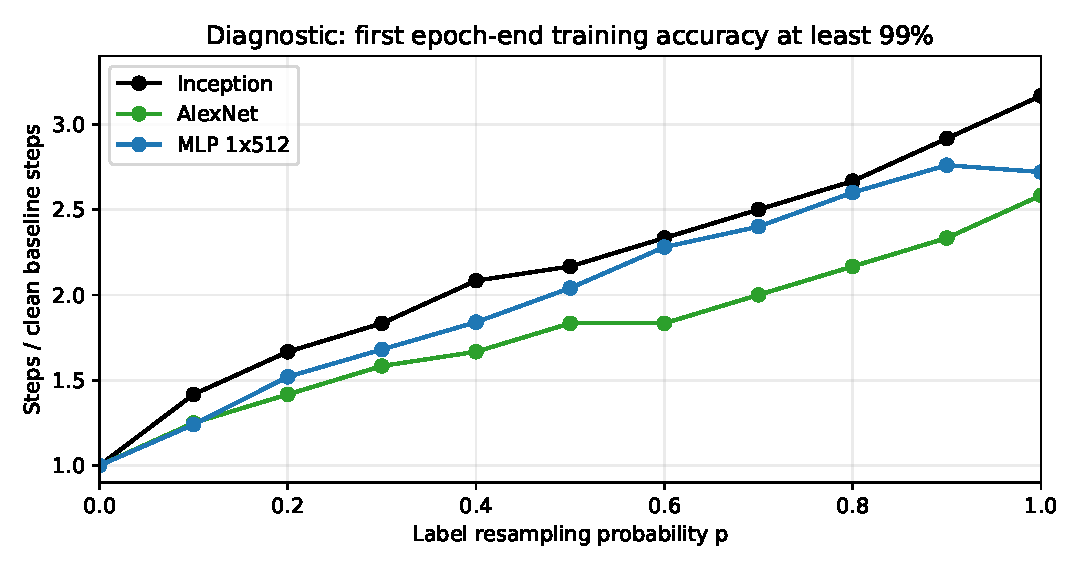
\includegraphics[width=0.88\textwidth]{report_assets/threshold_sensitivity.pdf}
\caption{Supplementary timing diagnostic at 99\% training accuracy, recomputed from the same selected histories. No retraining, interpolation of missing measurements, or smoothing was used. This threshold is not attributed to the authors.}
\label{fig:threshold-sensitivity}
\end{figure}

The threshold comparison directly demonstrates how the reported slowdown depends on the definition of fitting. It does not establish the authors' operational rule or isolate all causes of the mismatch. The continuation changes the schedule, and some relaxed-threshold MLP times also occur after that change. The rejected batch-size trial tests a second choice, but does not isolate initialisation or normalisation effects. A single seed leaves run-to-run variation unmeasured.

In panel (a), the loss curves retain oscillations after 100-update averaging. The paper gives no smoothing rule, so a different averaging window would change the presentation without verifying the original measurement convention. The saved plots retain their original smoothing.

All selected models fit both clean and fully random training labels to zero error. Their test accuracies range from 50.72\% to 86.52\% with clean labels and fall to about 10\% with fully random labels. These results support the paper's distinction between fitting arbitrary assignments and learning patterns that generalise. Exact-zero timing is strongly affected by residual errors, explaining important features of the reproduced panel (b). Its full ordering and magnitude remain unmatched under the declared criterion.

\subsection{Phase 4: status of an implementation comparison}

The implementation comparison remains pending because the Phase 3 code has not yet been saved in a Git commit. No new author-implementation access was undertaken for this revision. The results and diagnostics above belong to the Phase 3 attempt; the earlier source access is disclosed below.

\subsection{Code and interaction record}

The shared chat preserves the paper discussion and generated notebook revisions. Codex/IDE assistance converted the pasted code, launched the GPU runs, introduced the constant-rate continuation after the original schedule failed, and carried out the batch-size trials and later diagnostics. Execution was moved outside the chat to run and inspect the full experiments. The continuation and trial decisions are preserved in the local history rather than that shared conversation. This workflow does not fully meet the chat-interface requirement.

The LLM disclosed reading the authors' repository landing page and README, including example commands and sample output, before the reproduction was complete. It reported that it had not opened the Python implementation files. The shared page also lists \path{kobybibas/training_with_random_labels} as a search result. A second result is \path{google-research/heldout-influence-estimation}. Both include snippets. The web-tool outputs are redacted, so separate opening of those two repositories could not be verified. Framework documentation was also consulted. I subsequently instructed the LLM to avoid existing implementations.

The executed notebook retains the finished results. Decisions and failed trials are recorded in the assignment-root \path{reproduction_changes.md}; \path{README.md} beside the notebook provides run instructions. The supplementary calculations are reproducible with \path{report_diagnostics.py}, which reads saved histories and exports the full threshold grid with source-file hashes. No new training or author-code comparison was performed for the report revision.

\clearpage
\section{Critical review}

\subsection{Assessment of the paper}

The paper's controlled comparison is its main strength. The authors change the labels while keeping the architecture and training settings fixed. The same procedure then fits both correct labels and arbitrary assignments. Poor test accuracy with random labels is expected; reaching low training error with the unchanged procedure is the useful finding. The authors observe this behaviour across several architectures and input corruptions.

One control I would add is training on progressively smaller, correctly labelled datasets. The hypothesis is that corrupted supervision affects learning beyond the reduction in correct labels. At corruption probability $p$, the expected number of labels still equal to their original values is $n(1-0.9p)$. A clean subset of that size provides a count-matched control. With the architecture and optimisation budget controlled, higher test error under corruption would reject the simple explanation that performance depends only on the number of correct labels. The comparison should be repeated across subsets and seeds.

This count is not the amount of useful supervision: at $p=1$, about 10\% of random labels agree with the truth by chance, while the complete assignment is independent of the images. I would therefore also compare with a clean subset of expected size $n(1-p)$, matching the labels not selected for resampling. These controls separate different notions of reduced data. Similar training and test errors alone would not establish that reducing sample size and corrupting labels affect learning in the same way.

The theoretical interpretation is also limited. Fitting random labels shows why a worst-case bound based on the unrestricted model class can be loose. Bounds that account for the solution selected by training and the structure of the data could still be informative. The missing explanation is how training selects solutions that generalise in the tested nonlinear networks. The authors acknowledge this question and give a linear-model example of implicit bias, which leaves the nonlinear case open.

The ImageNet accuracy drop described in Section 1 shows that explicit regularisation still has a substantial practical effect. I read the results as evidence that regularisation contributes to performance alongside the architecture, data, and optimisation procedure. The authors also acknowledge its benefits.

One potential reporting inconsistency concerns fitting. Figure 1's caption says training error is zero, while Table 1 reports 99.82\% training accuracy for random-label AlexNet and 99.34\% for MLP 1$\times$512. If those table values describe the plotted checkpoints, test error exceeds the test-minus-training gap by 0.18 and 0.66 percentage points, respectively. The paper does not establish that they are the same checkpoints, so this is a clarification request rather than proof that Figure 1 is incorrect. The operational convergence-time rule, batch size, initialisation, and repeated-run variation would also help assess the timing claim.

\subsection{Comparison with the OpenReview discussion}

Agreement. \href{https://openreview.net/forum?id=Sy8gdB9xx\&noteId=rJUCC0pQg}{Reviewer 1} asked why equally sized architectures generalise differently, and \href{https://openreview.net/forum?id=Sy8gdB9xx\&noteId=HJwljOv4x}{Reviewer 3} valued the empirical evidence while noting the limited explanation~\cite{openreview_archive}. These points agree with my assessment of the experiments' strength and the missing nonlinear mechanism. The \href{https://openreview.net/forum?id=Sy8gdB9xx\&noteId=HJJR_fQUg}{authors' response} also treated architecture-dependent generalisation as an open question.

Difference in interpretation. \href{https://openreview.net/forum?id=Sy8gdB9xx\&noteId=B1nh-uNVl}{Reviewer 2} strongly endorsed the paper's criticism of classical complexity measures. My conclusion is narrower: unrestricted model-class capacity is insufficient, while bounds sensitive to the data and trained solution remain possible. These three official reviews were posted in December 2016, with ratings 10, 9, and 10 for Reviewers 1, 2, and 3.

Additional points. In a \href{https://openreview.net/forum?id=Sy8gdB9xx\&noteId=S1zRtYaBG}{public comment dated 30 January 2018}, Thomas Dietterich argued that roughly tripling the fitting time is meaningful and proposed early stopping as a capacity restriction. That proposal goes beyond my stopping-threshold diagnostic: it changes how long training runs rather than how fitting time is measured. Reviewer 1 also suggested testing prediction stability with dropout at inference, and Reviewer 3 requested clarification of the linear/kernel classification targets. Those were not controls in my assessment. Conversely, I did not find the smaller-clean-dataset control explicitly proposed in the three official reviews. Dietterich's later public comment is separate from those official reviews.

\noindent Access disclosure. The archived public discussion also contained a short illustrative nearest-neighbour/random-forest code example. It was encountered during this review comparison, after the reproduction runs, and was not used to modify the notebook or results. No neural-network implementation was consulted during this comparison.

\begin{thebibliography}{2}
\bibitem{zhang2017}
Chiyuan Zhang, Samy Bengio, Moritz Hardt, Benjamin Recht, and Oriol Vinyals.
\newblock Understanding deep learning requires rethinking generalization.
\newblock \emph{International Conference on Learning Representations}, 2017.
\bibitem{openreview_archive}
OpenReview. Official reviews, author response, and public discussion for paper \texttt{Sy8gdB9xx}.
\newblock \href{https://openreview.net/forum?id=Sy8gdB9xx}{Original discussion}; accessed through the
\href{https://github.com/xcfcode/openreview_spider/blob/b232dbcbbee6a7a39415c2ea046058e9dcd82e1e/res/Sy8gdB9xx.json}{archived OpenReview records}, 22 October 2026.
\end{thebibliography}

\end{document}
